\newpage
\changeindent{0cm}
\section{数値実験}
\label{sec:exp}
\changeindent{2cm}


\changeindent{0cm}
\subsection{提案手法:DARTS}
\label{sec:exp.01}
\changeindent{2cm}


\begin{table}[t]
  \begin{center}
    \caption{各アーキテクチャの精度}
		\vspace{3mm}
    \begin{tabular}{|c|c|c|c|c|c|}\hline
    \multicolumn{2}{|c|}{\textbf{architecture}} & \textbf{\begin{tabular}[c]{@{}c@{}}test accuracy\\ (\%)\end{tabular}} & \textbf{\begin{tabular}[c]{@{}c@{}}param\\ (M)\end{tabular}} & \textbf{\begin{tabular}[c]{@{}c@{}}number of\\ shortcuts\end{tabular}} & \textbf{\begin{tabular}[c]{@{}c@{}}random architect\\ accuracy (\%)\end{tabular}} \\ \hline
    \multirow{3}{*}{\begin{tabular}[c]{@{}c@{}}method A\end{tabular}} & 50 epoch & 93.70 $\pm$ 0.22 & 21.06 $\pm$ 0.07 & 12.7 $\pm$ 1.4 & 93.60 $\pm$ 0.15 \\ \cline{2-6}
     & 100 epoch & 94.02 $\pm$ 0.12 & 21.50 $\pm$ 0.11 & 18.2 $\pm$ 0.9 & 93.67 $\pm$ 0.14 \\ \cline{2-6}
     & 150 epoch & 93.90 $\pm$ 0.17 & 21.57 $\pm$ 0.25 & 18.9 $\pm$ 0.6 & 93.64 $\pm$ 0.09 \\ \hline
    \multirow{3}{*}{\begin{tabular}[c]{@{}c@{}}method B\end{tabular}} & 50 epoch & 93.57 $\pm$ 0.19 & 20.45 $\pm$ 0.09 & 5.8 $\pm$ 1.2 & 93.36 $\pm$ 0.19 \\ \cline{2-6}
     & 100 epoch & 93.93 $\pm$ 0.08 & 20.73 $\pm$ 0.10 & 9.8 $\pm$ 1.0 & 93.47 $\pm$ 0.17 \\ \cline{2-6}
     & 150 epoch & 93.92 $\pm$ 0.12 & 20.76 $\pm$ 0.15 & 10.6 $\pm$ 1.0 & 93.48 $\pm$ 0.15 \\ \hline
    \multicolumn{2}{|c|}{baseline (VGG19)} & 93.03 $\pm$ 0.10 & 20.04 & 0 & - \\ \hline
    \end{tabular}
    \label{tab:accg}
  \end{center}
\end{table}


\begin{figure}[t]
  \begin{center}
    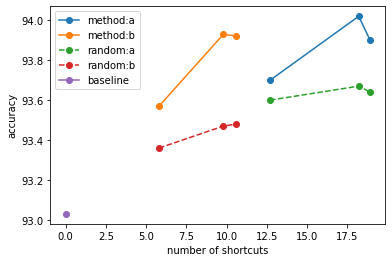
\includegraphics[clip,width=10cm]{./fig/short.png}
  \end{center}
  \caption{ショートカット数に対する精度}
  \label{fig:short}
\end{figure}
\begin{figure}[t]
  \begin{center}
    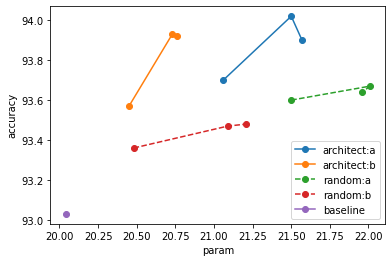
\includegraphics[clip,width=10cm]{./fig/param.png}
  \end{center}
  \caption{パラメータ数に対する精度}
  \label{fig:param}
\end{figure}

表 \ref{tab:accg} に各構成手法におけるテストデータの精度を示す.
図 \ref{fig:short}, \ref{fig:param} には
表 \ref{tab:accg} の精度に対するショートカット数とパラメータ数の関係を図示する.
最も性能が高かったのは100 epoch 時点の手法Aで94.02 \%(baseline+0.99\%)となり,
100 epoch 時点の手法Bは93.93 \%(baseline+0.90\%)となった.
しかしランダム手法と比較すると, 手法Aは+0.35\%, 手法Bは+0.46\%となり,
図 \ref{fig:param} を参照しても少ないパラメータ数でより有効に探索できているのは手法Bと言える.

また100 epoch時点と150 epoch時点を比較すると, 学習によって性能が悪化している.
問題に対して過度に適合していることが原因であると考えられる.

探索時間は150 epochでおよそ 5 GPU hours を要したが, DARTSと比べ演算子を探索していないことや.
最適な重み $w^*$ の近似を1次下げていることで高速になったと思われる.




\clearpage\newpage
\changeindent{0cm}
\subsection{提案手法:DARTS+TDGA}
\label{sec:exp.02}
\changeindent{2cm}


\begin{figure}[t]
  \begin{center}
    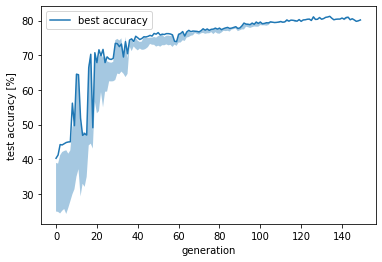
\includegraphics[clip,width=10cm]{./fig/04.exp/acc_tdga.png}
  \end{center}
  \caption{TDGA精度}
  \label{fig:acc_tdga}
\end{figure}

\begin{figure}[t]
  \begin{center}
    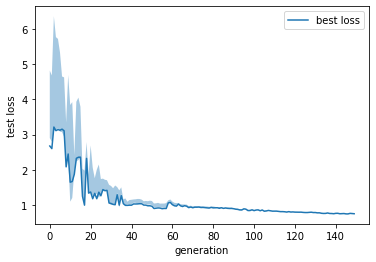
\includegraphics[clip,width=10cm]{./fig/04.exp/loss_tdga.png}
  \end{center}
  \caption{TDGA loss}
  \label{fig:loss_tdga}
\end{figure}

\begin{figure}[t]
  \begin{center}
    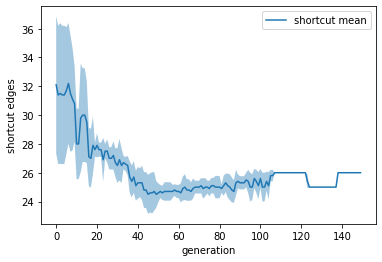
\includegraphics[clip,width=10cm]{./fig/04.exp/edge_tdga.png}
  \end{center}
  \caption{TDGA edge}
  \label{fig:edge_tdga}
\end{figure}

\begin{figure}[t]
  \begin{center}
    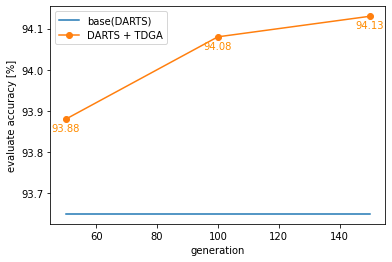
\includegraphics[clip,width=10cm]{./fig/04.exp/eval_tdga.png}
  \end{center}
  \caption{TDGA eval}
  \label{fig:eval_tdga}
\end{figure}
